\section{DNS database and problem setup}

The DNS database consists of four simulations of an inlet-outlet configuration of 
statistically-planar turbulent premixed lean methane flames evolving in a box with periodic 
lateral boundary conditions.
%
The thermodynamic variables of the simulation are initialized from a one-dimensional
methane-air laminar flame solution.
%
The laminar flame solution was obtained using the 16 species/35 reactions mechanism of Smooke and Giovangigli and \cite{smooke1991reduced} under the standard atmospheric pressure, 
a fresh gases state temperature $T_u\approx298K$ and an equivalence ratio $\phi=0.7$.
% 
Under these conditions, the unstrained flame speed $S_L\approx0.18cm/s$ and the thermal flame thickness
, determined by the maximum temperature gradient, \ie. $\delta_L=(T_b-T_u)/\max(|\nabla T|)\approx 660 \mu m$, where $T_b$ the burnt gases temperature is about $1840K$.
%
For each case of the DNS database, the extracted thermodynamic profiles are superimposed onto a turbulent velocity field obtained from a preliminary inert homogeneous isotropic turbulent (HIT) simulation on a periodic box of size $L^3$.
%
The latter corresponds to the establishment of turbulence starting from synthetic turbulent fluctuations
prescribed by a \citet{passot1987numerical} energy spectrum.
%
In this auxiliary HIT computation, the turbulence was maintained and driven to establish quasi-stationary state by introducing a zero-mean time-dependent a long-wavenumber forcing term \cite{aspden2009analysis,aspden2011turbulence} into the momentum equation.
%
In addition to its use as an initial velocity field in the reactive simulation, the obtained HIT
solution is used to feed the inflow turbulent velocity fluctuations.
%
These fluctuations are injected using an active control method \cite{hassanaly2015influence} based on the
strategy introduced by \citet{bell2007active} consisting of a dynamic adjustment of the inflow
conditions to maintain the flame mean location in the centre of the computational domain.
%
To avoid the altercation of the  flame-turbulence interaction, the application of the same 
long-wavenumber forcing strategy is discarded in the burnt mixture and in the flame zone 
restricted to the unburned gases side up to one laminar flame thickness before the
flame leading edge.
%
For all the considered cases, the computational domain size is $2L\times L\times L$ where
the computational domain characteristic size along the crosss-stream, \ie $y$ and $z$, directions
 $L$ is about $8 ~\delta_L$ .

The parameter of interest of the current DNS database, is the ratio between the turbulent 
fluctuations intensity $u^{\prime}$ and the unstrained laminar flame speed $S_L$.
%
The four cases considered, herein, correspond to a variation of the parameter $\Upsilon\equiv 
u^{\prime}/S_L$ between 2.5-150 and correspond to the well stirred reactor and broken reaction
zones in the Borghi diagram as shown by \autoref{fig:borghi}.
%
Independently from the considered intensity, The integral length scale $l_t$ is set to be in the
same order as the thermal thickness, such that the ratio $\Lambda \equiv l_t/\delta_L\approx 1.75$.
%
As shown in \autoref{tab:dns_details}, the initial Damk\"ohler, $Da=\Lambda/\Upsilon$, which is the ratio between
the chemical and the integral time scales is in the range 0.012--0.700.
%
The Karlovitz, Ka$=(\Upsilon^3/\Lambda)^{1/2}$, which measures the relative turbulence strength 
to the flame corresponds to the range 3.0--1390.
%
The corresponding range of the turbulent Reynold number, $\mathrm{Re}_t=u^{\prime}l_t/\nu$, based on the integral length scale is approximatively 32--1950, where $\nu$ is the kinematic viscosity.
%
The grid resolution, $N$, is adjusted so that, at least, 16 computational cells are within the
thermal flame thickness, and ensuring that the ratio of the Kolmogorov scale $\eta=l_t/(\mathrm{Da~Ka})^2$ 
over the the discretization step $\Delta x$  is kept larger than 1.7.

\begin{figure}[htbp]
    \centering
    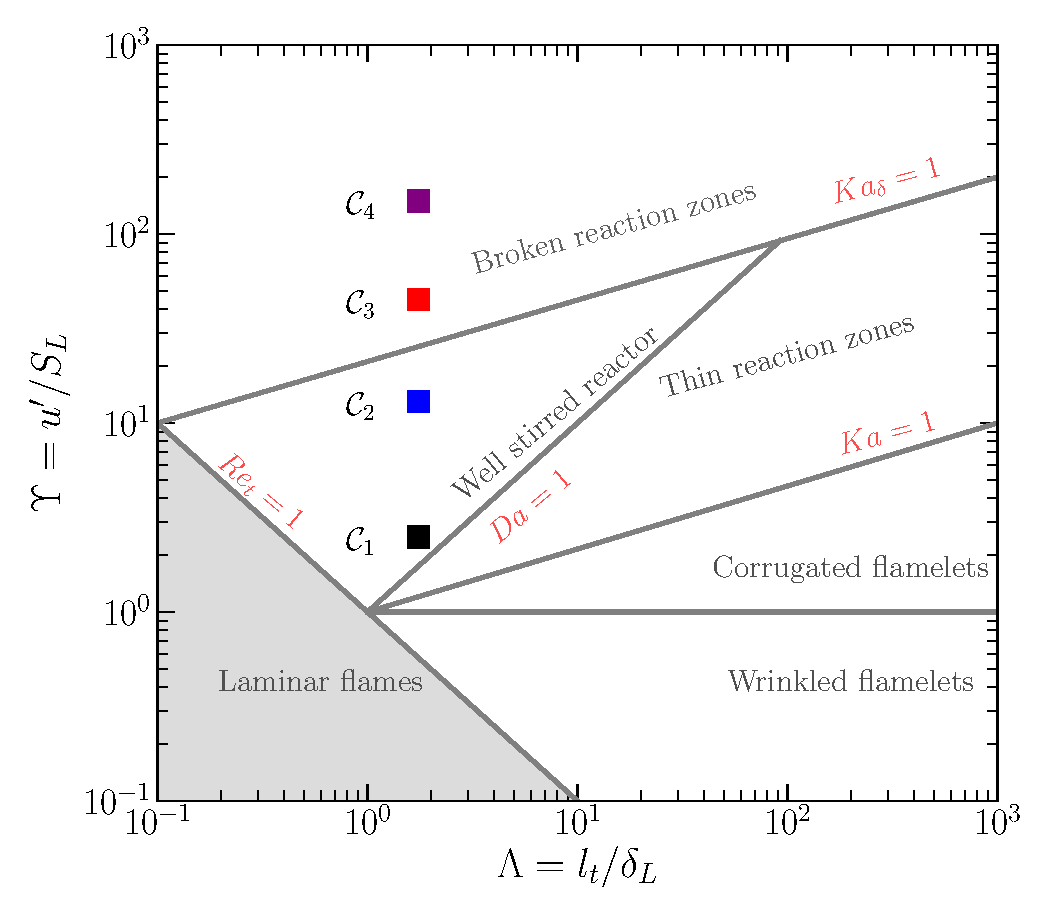
\includegraphics[width=0.7\textwidth]{./figs/borghi.pdf}
    \caption{Borghi combustion diagram showing the location of the cases $\mathcal{C}_1--\mathcal{C}_4$.
    Herein, Da and Ka are the Damk\"ohler and Karlovitz numbers, Re is the Reynolds number which is
    equal to (Da Ka)$^2$, and $Ka_\delta$ is the Karlovitz number based on the reaction zone thickness
    and approximated as $Ka_\delta\sim \mathrm{Ka}/100$.}
    \label{fig:borghi}
\end{figure}


\begin{table}[]
\centering
\begin{tabular}{ccrcrr}
\toprule
Case & $N$ & $\Upsilon$ & $Da$ & $Ka$ & $Re_t$ \\
\midrule
$\mathcal{C}_1$ & 128 & 2.5 & 0.700 & 3.0 & 32.5 \\
$\mathcal{C}_2$ & 128 & 13 & 0.135 & 35 & 169 \\
$\mathcal{C}_3$ & 256 & 45 & 0.039 & 228 & 584.5 \\
$\mathcal{C}_4$ & 512 & 150 & 0.012 & 1389 & 1948.4\\
\bottomrule
\end{tabular}
\caption{Grid resolution and initial turbulent-to-laminar flame speed ratio $\Upsilon \equiv u^{\prime}/S_L$,  Damk\"ohler, Da$=\Lambda/\Upsilon$, Karlovitz Ka$=(\Upsilon^3/\Lambda)^{1/2}$ and
 turbulent Reynolds number $\mathrm{Re}_t=u^{\prime}l_t/\nu$ used in the current DNS database.}
\label{tab:dns_details}
\end{table}
